\documentclass[UTF8,fontset=fandol,11pt,a4paper]{ctexart}
\usepackage[margin=2.15cm,headheight=15pt,headsep=11pt,footskip=22pt]{geometry}
\usepackage{amsmath,amssymb,newtxtext,newtxmath,booktabs,tabularx,graphicx,enumitem,xurl,fancyhdr}
\usepackage[unicode,hidelinks]{hyperref}
\graphicspath{{../Figures/}}
\makeatletter
\setlength{\@fptop}{0pt}\setlength{\@fpsep}{18pt}\setlength{\@fpbot}{0pt plus 1fil}
\makeatother
\setlength{\parindent}{2em}\setlength{\parskip}{3pt}\setlength{\emergencystretch}{2em}
\linespread{1.08}\renewcommand{\arraystretch}{1.15}
\setlist[itemize]{leftmargin=1.5em,itemsep=3pt,topsep=3pt}
\setlist[enumerate]{leftmargin=1.7em,itemsep=4pt,topsep=3pt}
\ctexset{section={format=\large\bfseries,beforeskip=1.2ex,afterskip=.7ex},subsection={format=\normalsize\bfseries,beforeskip=1ex,afterskip=.5ex}}
\pagestyle{fancy}\fancyhf{}\fancyhead[L]{\small B：多岭参数平均与信号谱对齐}\fancyhead[R]{\small 2026 年 11 月 4 日}\fancyfoot[C]{\small\thepage}
\hypersetup{pdftitle={多岭参数平均的风险、信号谱对齐与选权代价},pdfauthor={高维统计课程项目}}
\begin{document}

\begin{center}
{\LARGE\bfseries 多岭参数平均的风险、信号谱对齐与选权代价\par}
\vspace{6pt}
{\large B 计划首轮研究报告与复现实验\par}
\vspace{4pt}{\small 2026 年 11 月 4 日\quad 代码、原始结果与数学证明配套交付}
\end{center}
\begin{abstract}
本研究从同一训练数据、多个正则参数的岭回归平均出发，建立一般系数先验下的精确条件风险矩阵，
给出各向同性情况下可由单参数 resolvent 差商计算的高维极限，
并区分连续单岭基准、平均家族的可达收益和训练数据选权造成的损失。
主实验包含 $18$ 个配置、每配置 $100$ 次独立重复，共 $1\,800$ 份训练数据、$21\,600$ 条方法记录；
另以 $300$ 份数据验证普通 GCV 的极限反例，以 $720$ 份数据验证有界谱下的确定性等价。
各向同性控制中，连续单岭与先验平均 oracle 混合风险一致；
弱谱方向的信号方差提高时，凸平均存在小幅结构收益；强谱方向更突出时，受约束负权重可扩大可达收益。
但本次实际选权没有实现这些 oracle 收益：校正与 LOO 显著改善普通 GCV 平均，仍未优于单岭调参。
这支持将后续问题聚焦于稳定选权，而不能宣称已提出普遍优于岭回归的新方法。
\end{abstract}

\section{已完成的工作与主要结论}
\begin{enumerate}
\item \textbf{风险公式已实现并核验。}一般先验协方差 $\Psi$ 下直接计算完整交叉风险，保留 $p>n$ 的样本零空间；
各向同性极限的方差交叉项包含 $S=X^\mathsf TX/n$，没有将其错误替换为偏差项。
\item \textbf{信号结构确实影响平均的可达收益，但幅度小。}
当 $b-a=-0.3$，六个配置的凸平均条件风险收益范围为
$0.000904$ 至 $0.002874$；
当 $b-a=+0.3$，负权重 oracle 的收益范围为
$0.000457$ 至 $0.001372$。
这些是总风险的绝对差，不能误读成百分数。各向同性控制的最大逐次风险偏差小于 $10^{-12}$。
\item \textbf{普通 GCV 的失准有明确代数机制。}
普通聚合 GCV 与逐候选交叉残差准则可由同一个单纯形二次规划求解，
但前者将解按 $1/(1-\mathrm{df}_j/n)$ 再加权，可能放大高自由度候选。
两者最小分数相同，并不意味着拟合出的模型或实际风险相同。
\item \textbf{有限样本选权仍是主要代价。}
在全部 $18$ 个配置中，本次交叉残差、LOO 及受约束负权重选权的平均风险仍高于连续单岭 oracle；
不能将固定权重校准有效直接解释为自适应选权已经达到最优。
\end{enumerate}

本文的风险恒等式、代数推导和模拟用于课程项目的可核验推广。
多岭参数平均、source condition、正则外推与交叉风险校正均已有相关研究\cite{zhao,richards,bach,bellec}；
本报告不据此宣称论文级原创性已确认。

\clearpage
\section{实验设计、信息范围与计算方法}
总体特征基中令 $\Sigma=\operatorname{diag}(\mu_1,\ldots,\mu_p)$，
系数先验为 $\beta\sim N(0,\Psi)$，$\Psi=\operatorname{diag}(\psi_1,\ldots,\psi_p)$，
训练特征行为 $N(0,\Sigma)$，噪声为独立 $N(0,1)$。
主实验固定 $n=100$、$p/n\in\{0.8,1,1.5\}$、$a\in\{1.5,2\}$，并取
\begin{equation}\label{eq:experiment_population}
 \mu_i=\frac{p\,i^{-a}}{\sum_{\ell=1}^p\ell^{-a}},\qquad
 \psi_i=\frac{i^{a-b}}{\sum_{\ell=1}^p\mu_\ell\ell^{a-b}},\qquad
 b-a\in\{-0.3,0,0.3\}.
\end{equation}
于是 $\operatorname{tr}\Sigma=p$，$\mathbb E[\beta^\mathsf T\Sigma\beta]=1$，总体预测信噪比始终为 $1$；
$b=a$ 时 $\Psi=I_p/p$。
主实验的幂律谱属于固定有限维机制研究；有界谱渐近验证单独进行，未混用理论适用范围。

候选参数为 $[10^{-4},10^2]$ 上 $21$ 个对数等距点，再加入 $p/n$（去重后 $21$ 或 $22$ 点），
确保各向同性时已包含精确最优单岭参数。
连续单岭 oracle 在 $[10^{-6},10^4]$ 上先检查 $101$ 个对数点，再精化所有检测到的局部极小值；
各向同性时直接使用 $\lambda_*=p/n$。它是宽区间内的数值基准，未证明任意各向异性风险曲线全局单峰。
负权重同时约束 $\boldsymbol1^\mathsf T\pi=1$、$\lVert\pi\rVert_1\le3$。

\textbf{信息范围。}先验平均 oracle 只使用 $X$ 以及已知的 $\Sigma,\Psi$；
实际的 Ridge-GCV、普通 GCV 平均、交叉残差平均及 LOO 平均只使用 $X,y$。
广义 Bayes oracle 还知道真实各向异性先验，作为更宽方法类的参照。
真实 $\beta$ 只进入独立评估
\begin{equation}\label{eq:experiment_evaluation}
 R_{\mathcal D}=1+(\widehat\beta-\beta)^\mathsf T\Sigma(\widehat\beta-\beta),
\end{equation}
不参与这些算法的训练。该式将新测试点精确积分掉，因此没有额外有限测试集噪声。
各配置内所有方法共享同一训练数据，差值标准误按配对重复计算；根种子为 $202611041$，
主实验、MP 验证、确定性等价验证采用不同种子分支。
图中误差线为 $\pm1$ 个 Monte Carlo 标准误，表中为均值 $\pm\mathrm{SE}$。
配对 $95\%$ 区间为正态近似的逐项描述，没有多重比较校正。

\clearpage
\section{平均家族的结构收益}
表\ref{tab:oracle}报告给定设计后、对系数与训练噪声平均的风险。
收益定义为连续单岭风险减去对应平均风险；正值表示平均更好。
该目标适用于只依赖设计与生成参数的 oracle，不能用来替代数据自适应选权的实际评估。
\begin{table}[htbp]\centering\small
\caption{全部主配置的条件 oracle 收益；后两列以 $10^{-3}$ 为单位}\label{tab:oracle}
\renewcommand{\arraystretch}{1.12}
\begin{tabular}{cccccc}\toprule
$a$ & $p/n$ & $b-a$ & 连续单岭总风险 & 凸平均收益 $\pm\mathrm{SE}$ & 负权平均收益 $\pm\mathrm{SE}$\\\midrule
1.5 & 0.8 & $-0.3$ & $1.3057$ & $2.354\pm0.015$ & $2.356\pm0.015$ \\
1.5 & 0.8 & $+0.0$ & $1.2131$ & $0.000\pm0.000$ & $0.000\pm0.000$ \\
1.5 & 0.8 & $+0.3$ & $1.1492$ & $-0.343\pm0.002$ & $1.280\pm0.007$ \\
1.5 & 1 & $-0.3$ & $1.3277$ & $2.599\pm0.015$ & $2.601\pm0.015$ \\
1.5 & 1 & $+0.0$ & $1.2224$ & $0.000\pm0.000$ & $0.000\pm0.000$ \\
1.5 & 1 & $+0.3$ & $1.1519$ & $-0.087\pm0.001$ & $1.303\pm0.009$ \\
1.5 & 1.5 & $-0.3$ & $1.3620$ & $2.874\pm0.014$ & $2.876\pm0.014$ \\
1.5 & 1.5 & $+0.0$ & $1.2357$ & $0.000\pm0.000$ & $0.000\pm0.000$ \\
1.5 & 1.5 & $+0.3$ & $1.1577$ & $-0.358\pm0.002$ & $1.372\pm0.009$ \\
2 & 0.8 & $-0.3$ & $1.1683$ & $0.904\pm0.006$ & $0.904\pm0.006$ \\
2 & 0.8 & $+0.0$ & $1.1175$ & $0.000\pm0.000$ & $0.000\pm0.000$ \\
2 & 0.8 & $+0.3$ & $1.0865$ & $-0.155\pm0.001$ & $0.458\pm0.004$ \\
2 & 1 & $-0.3$ & $1.1723$ & $0.913\pm0.005$ & $0.914\pm0.005$ \\
2 & 1 & $+0.0$ & $1.1186$ & $0.000\pm0.000$ & $0.000\pm0.000$ \\
2 & 1 & $+0.3$ & $1.0869$ & $-0.036\pm0.001$ & $0.457\pm0.004$ \\
2 & 1.5 & $-0.3$ & $1.1792$ & $0.930\pm0.006$ & $0.930\pm0.006$ \\
2 & 1.5 & $+0.0$ & $1.1211$ & $0.000\pm0.000$ & $0.000\pm0.000$ \\
2 & 1.5 & $+0.3$ & $1.0873$ & $-0.160\pm0.001$ & $0.459\pm0.004$ \\
\bottomrule\end{tabular}
\par\vspace{3pt}{\footnotesize 每格 $100$ 份独立设计。均值与标准误按逐次配对风险差计算。
极微小的负权额外收益仍须与优化间隙比较；例如弱谱方向下负权相对凸平均约 $10^{-6}$ 量级的差异不作实质改善结论。}
\end{table}
\textbf{各向同性控制。}当 $b=a$，连续单岭、包含其参数的凸平均及负权平均 oracle 均恢复同一风险，
符合最优线性/Bayes 基准。
当 $b<a$，凸平均在本次六个配置中有严格的正收益；当 $b>a$，有限凸候选族未胜过连续单岭，
但受约束负权重获得正收益。
负的凸平均收益混合了候选网格与滤波器形状限制，不能据此证明无限密网格的凸平均也存在严格劣势。
这些观察是本次有限参数范围内的机制证据，不是关于任意 source condition 的“当且仅当”定理。

\textbf{排除网格混杂的补充诊断。}对相同的 $1\,800$ 个设计，将各自连续最优单岭参数再加入 oracle 候选，
只重新求解凸平均；它不改变实际选权方法，也不增加独立数据量。
当 $b-a=+0.3$ 时，全部 $600$ 个增广凸平均解均回到该连续单岭顶点，收益在机器精度内为零。
因此原表中这些配置的轻微负收益应归于有限网格；现有诊断支持“增广候选凸平均没有额外收益”，
仍不构成关于任意正则参数连续混合的全局不可能性定理。
完整逐次结果见 \texttt{anchor\_diagnostic.csv}。

\begin{figure}[p]\centering
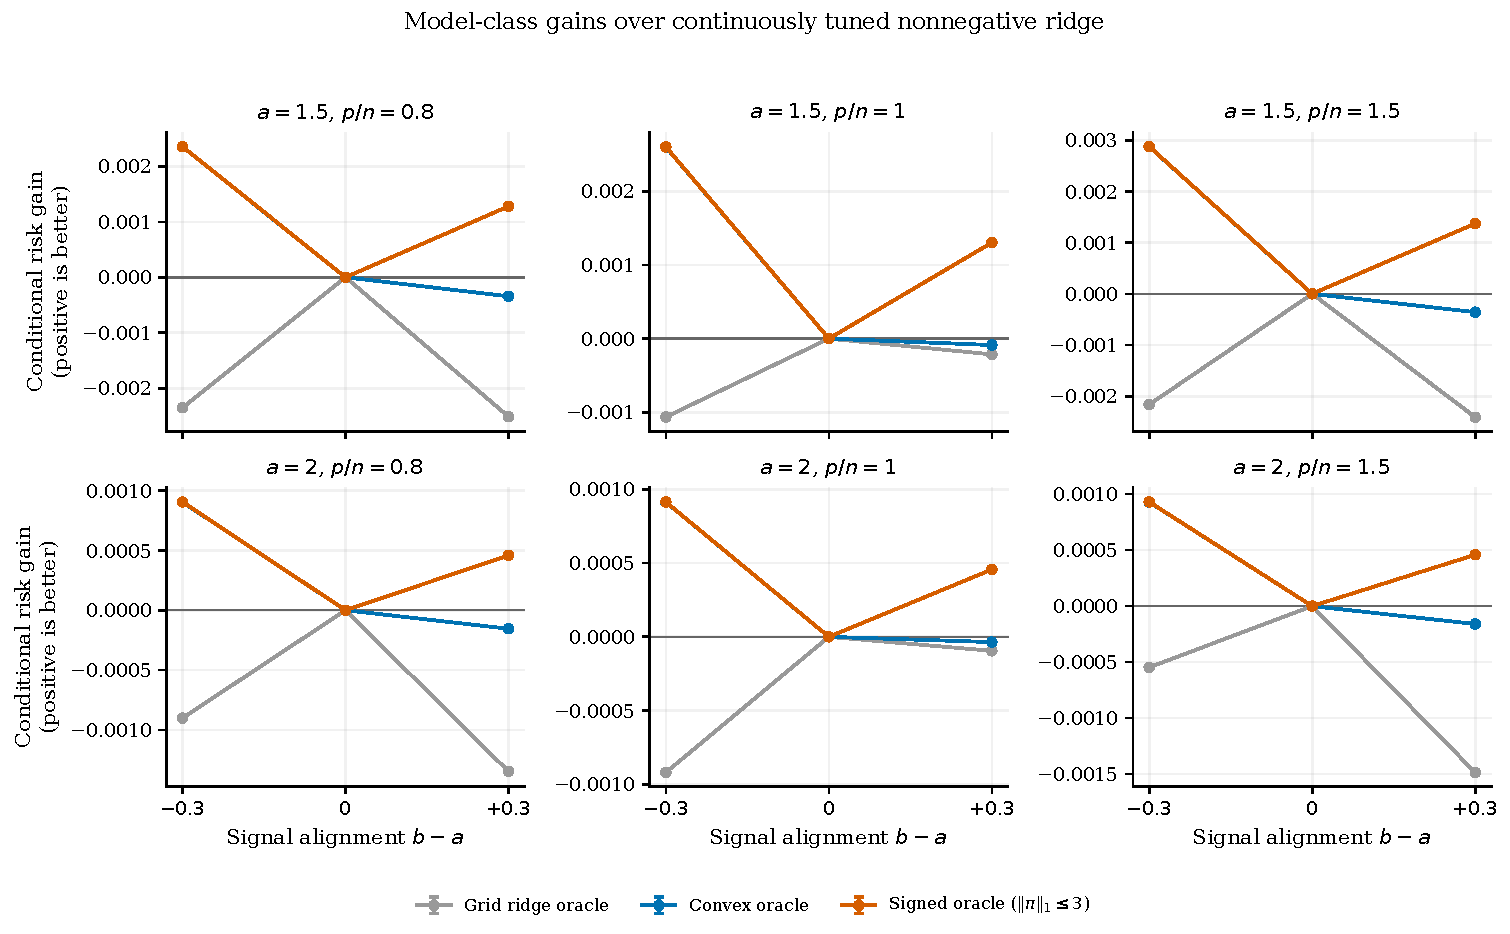
\includegraphics[width=\textwidth]{oracle_gains.pdf}
\caption{相对连续单岭的条件风险收益。横轴为信号谱对齐差 $b-a$，
灰线为离散网格单岭，蓝线为凸平均，橙线为 $\ell_1\le3$ 的负权平均。
正值表示收益；误差线为配对均值的 $\pm1\mathrm{SE}$。部分误差线小于标记大小。}
\label{fig:oracle}
\end{figure}
\clearpage
\section{实际选权没有自动实现 oracle 收益}
以插值附近的配置 $a=1.5,p/n=1,b-a=-0.3$ 为例，表\ref{tab:actual}同时展示实际预测风险与训练内分数。
其余配置全部保存在原始和汇总 CSV，并见图\ref{fig:actual}。
即使使用完全相同的最小分数，普通 GCV 与交叉残差准则也可能给出风险截然不同的实际模型。
\begin{table}[htbp]\centering\small
\caption{代表配置的总预测风险与校准；$100$ 次配对重复}\label{tab:actual}
\renewcommand{\arraystretch}{1.2}
\begin{tabular}{lccc}\toprule
方法 & 总风险 $\pm\mathrm{SE}$ & 平均分数/平均风险 & 平均 $\lVert\pi\rVert_1$\\\midrule
连续单岭 oracle & $1.3345\pm0.0063$ & -- & -- \\
网格单岭 oracle & $1.3365\pm0.0064$ & -- & 1.000 \\
凸平均 oracle & $1.3319\pm0.0063$ & -- & 1.000 \\
负权平均 oracle & $1.3318\pm0.0063$ & -- & 2.067 \\
单岭 GCV & $1.3571\pm0.0075$ & 0.961 & 1.000 \\
普通 GCV 平均 & $4.1384\pm0.3845$ & 0.303 & 1.000 \\
交叉残差平均 & $1.4763\pm0.0290$ & 0.850 & 1.000 \\
LOO 平均 & $1.4179\pm0.0150$ & 0.894 & 1.000 \\
负权交叉残差平均 & $1.8692\pm0.0894$ & 0.605 & 3.000 \\
等权平均 & $1.9793\pm0.0209$ & 0.990 & 1.000 \\
最小范数 & $3.16\times10^{4}$（样本均值） & -- & -- \\
广义 Bayes oracle & $1.3308\pm0.0063$ & -- & -- \\
\bottomrule\end{tabular}
\par\vspace{3pt}{\footnotesize oracle 的已知生成参数风险不作为训练内分数。
最小范数在 $p=n$ 下的理论期望风险为无穷，样本均值仅作描述，不报告普通均值 SE。}
\end{table}

\textbf{可实现收益与估计代价。}交叉残差与 LOO 明显缓解了普通 GCV 平均的风险膨胀，
但仍未达到本次连续单岭基准；受约束负权重的实际选权反而更不稳定。
该结果与“扩大函数家族就能自动提高预测表现”的推断不一致。
校正矩阵能估计固定模型的风险，不意味着对许多权重取最小值后仍完全校准；
本次自适应分数普遍存在向下的选择偏差。
配对差值、比值的 Monte Carlo 标准误以及逐次权重均已保存，避免只比较独立组均值。
相对同样仅用训练数据调参的 Ridge-GCV，本次交叉残差平均与 LOO 平均均没有出现配对 $95\%$ 区间完全低于零的配置；
分别有 $12$ 个和 $11$ 个配置的区间完全高于零。
这些是未做多重校正的 Monte Carlo 描述，不能读作普适劣势定理。

\textbf{机制核验。}全部 $1\,800$ 次重复中，普通 GCV 权重均由交叉残差最优权重按命题 3 精确转换。
两种准则最小值的最大绝对差小于 $10^{-12}$，而预测风险可以相差很大。
这将“指标最小化成功”和“实际预测模型好”明确区分。
\begin{figure}[p]\centering
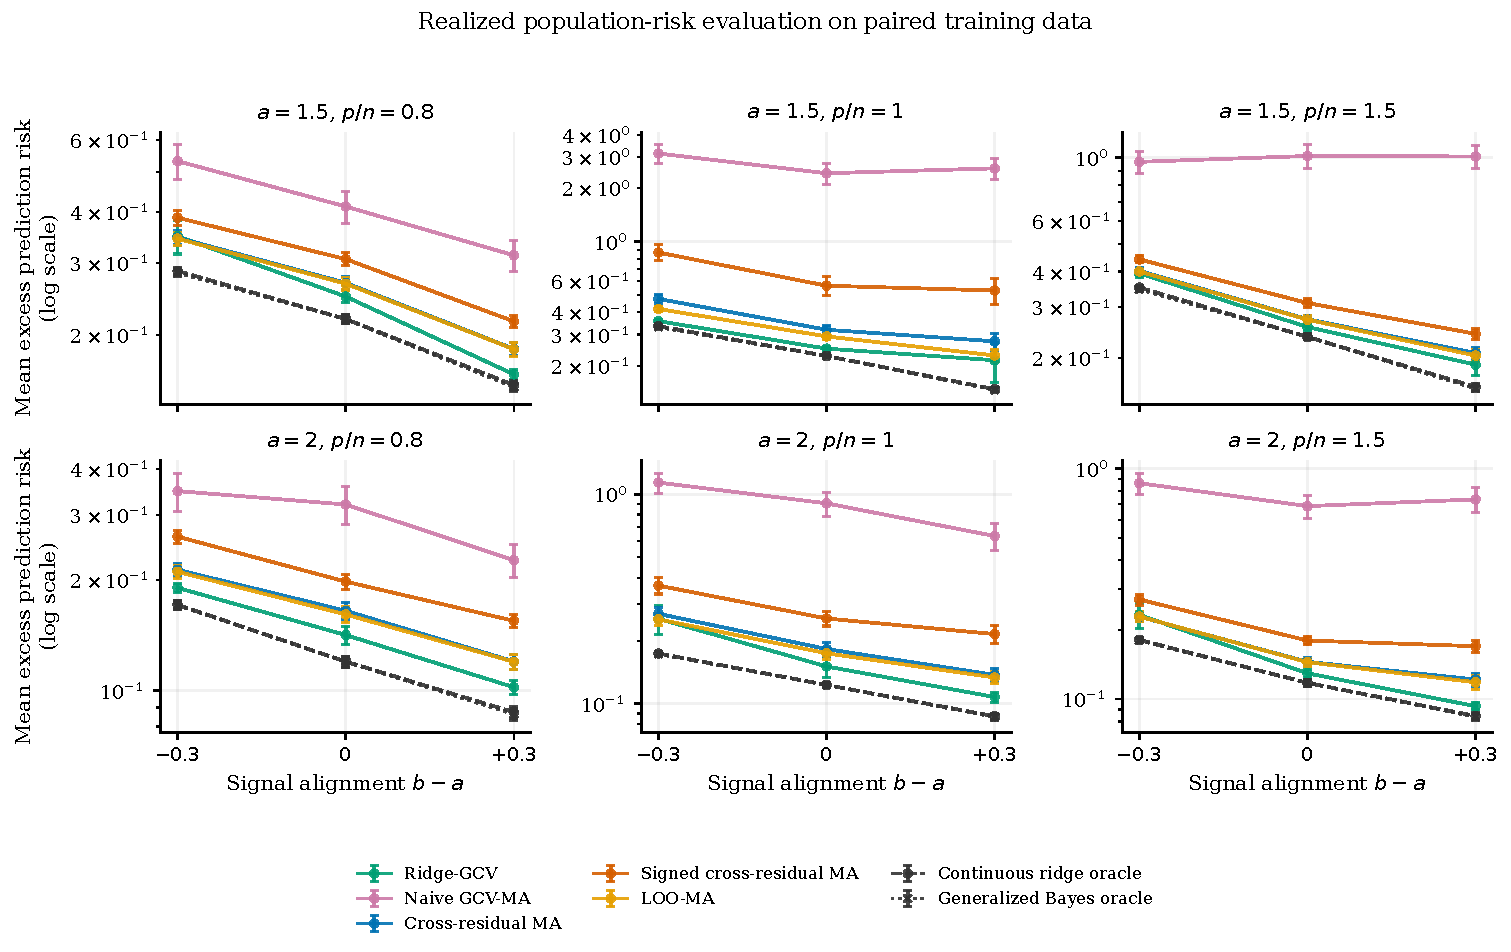
\includegraphics[width=\textwidth]{selected_risk.pdf}
\caption{所有主配置的实际平均超额风险，纵轴为对数尺度。
所有方法共享各次训练数据，oracle 曲线使用已知生成参数。
误差线为训练重复均值的 $\pm1\mathrm{SE}$。连续单岭与广义 Bayes 在各向同性控制中重合。}
\label{fig:actual}
\end{figure}
\begin{figure}[p]\centering
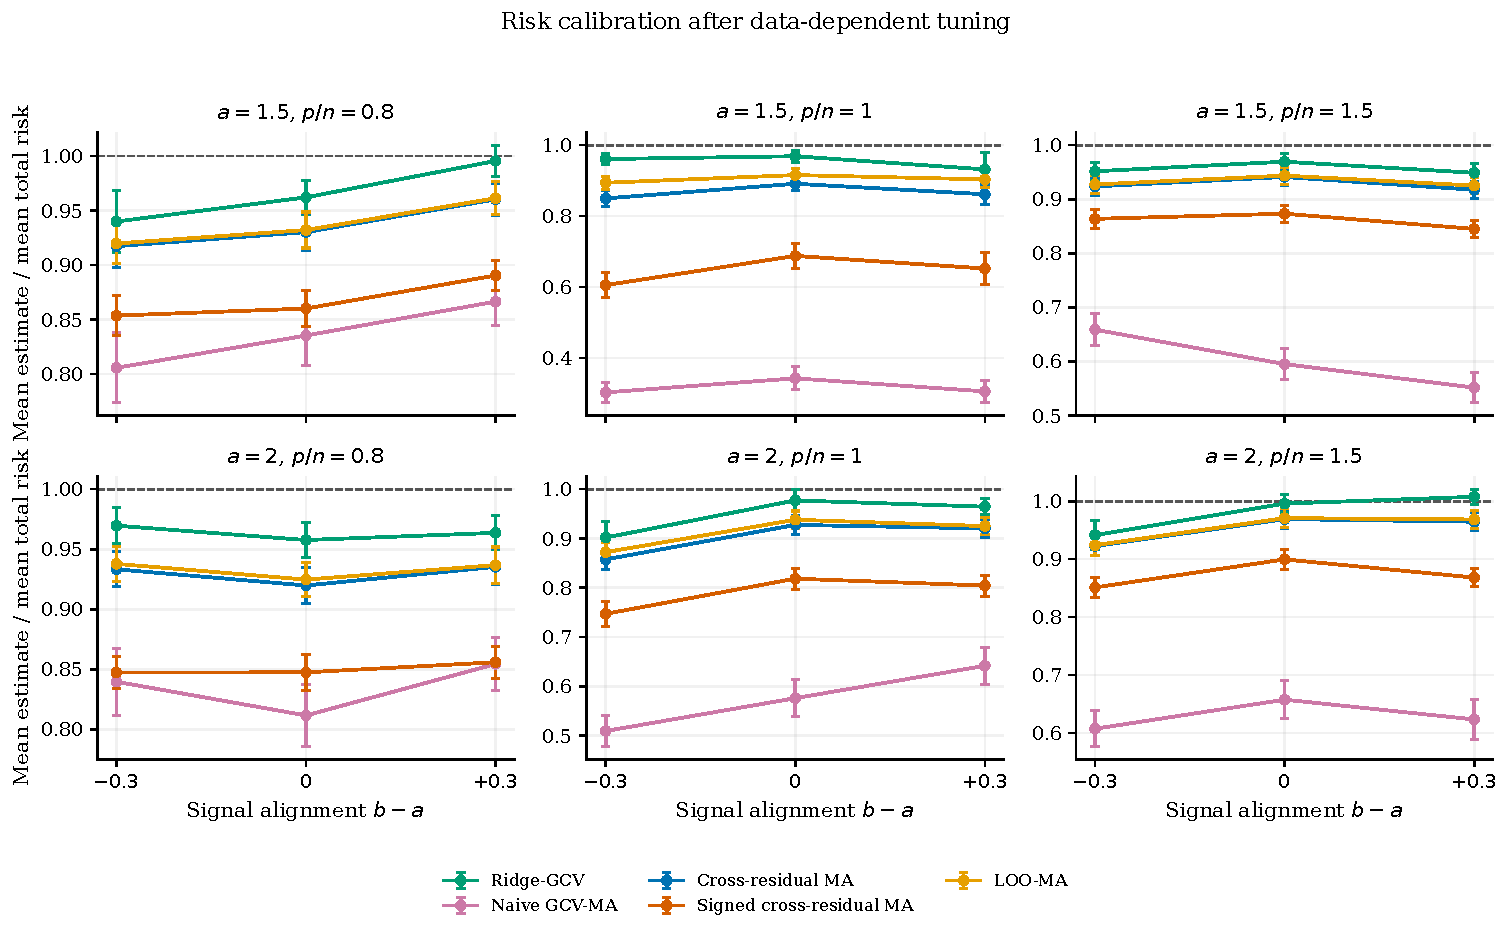
\includegraphics[width=\textwidth]{calibration.pdf}
\caption{自适应选权后的校准比，即训练内分数的重复均值除以独立评估总风险的重复均值。
虚线 $1$ 表示均值尺度校准；它不表示每份数据上都准确。误差线使用配对 delta 方法。}
\label{fig:calibration}
\end{figure}
\clearpage
\section{独立公式验证与数值审计}
\subsection{固定等权平均的 MP 反例}
取单位协方差、各向同性系数、噪声方差 $1$、$p=n$，比较两组固定候选参数。
每个规模 $n\in\{100,300,600\}$ 使用 $100$ 份独立数据；两组参数共享这些数据。
表\ref{tab:mp}展示 $n=600$ 的结果，与解析极限一致。
\begin{table}[htbp]\centering\small
\caption{固定等权平均：$n=600$ 的验证结果与理论极限}\label{tab:mp}
\renewcommand{\arraystretch}{1.2}
\begin{tabular}{cccccc}\toprule
参数对 & 实际风险 & 普通 GCV & 交叉残差 & 风险极限 & 普通 GCV 极限\\\midrule
$(0.1,1)$ & $1.7857$ & $1.6799$ & $1.7842$ & $1.7875$ & $1.6808$ \\
$(0.01,10)$ & $2.4359$ & $1.7721$ & $2.4293$ & $2.4435$ & $1.7700$ \\
\bottomrule\end{tabular}\end{table}
此处没有优化权重，所以固定权重的 GCV 失准与数据自适应选择偏差已经被分开。
这也说明不能仅凭单岭 GCV 的一致性就推断平均后普通 GCV 一致。

\subsection{有界谱下的高维风险验证}
另取单位谱和等比例两块谱 $\{0.5,1.5\}$，$n\in\{100,200,400\}$、
$p/n\in\{0.8,1,1.5\}$，每配置 $40$ 次，共 $720$ 份独立设计。
比较单岭 $\lambda=1$ 与三参数 $\lambda=(0.1,1,10)$、权重 $(0.2,0.5,0.3)$ 的固定平均。
以实际样本设计的精确先验平均风险作为参照，使用总体谱方程计算确定性等价。
在 $n=400$ 的 $12$ 个方法配置中，组均值的最大绝对相对偏差为 $0.028\%$。

\subsection{复现与求解精度}
保存结果共含 $1\,800$ 个不同主实验种子。
每个配置的首个重复均独立重跑，风险与保存值的最大绝对差为 $0.00$。
全部方法记录的求解检查通过，最大归一化一阶间隙为 $1.91\times10^{-5}$，
最大约束误差为 $7.99\times10^{-15}$。
一次初始负权重求解未达到间隙阈值，已使用相同数据种子进一步求解并重新核验；没有替换训练数据。
一般先验风险与直接矩阵逆计算、$p>n$ 零空间、显式删点 LOO、Bayes 基准及 GCV 换元均有独立测试。
检验代码与机器可读审计记录一起交付。
\begin{figure}[p]\centering
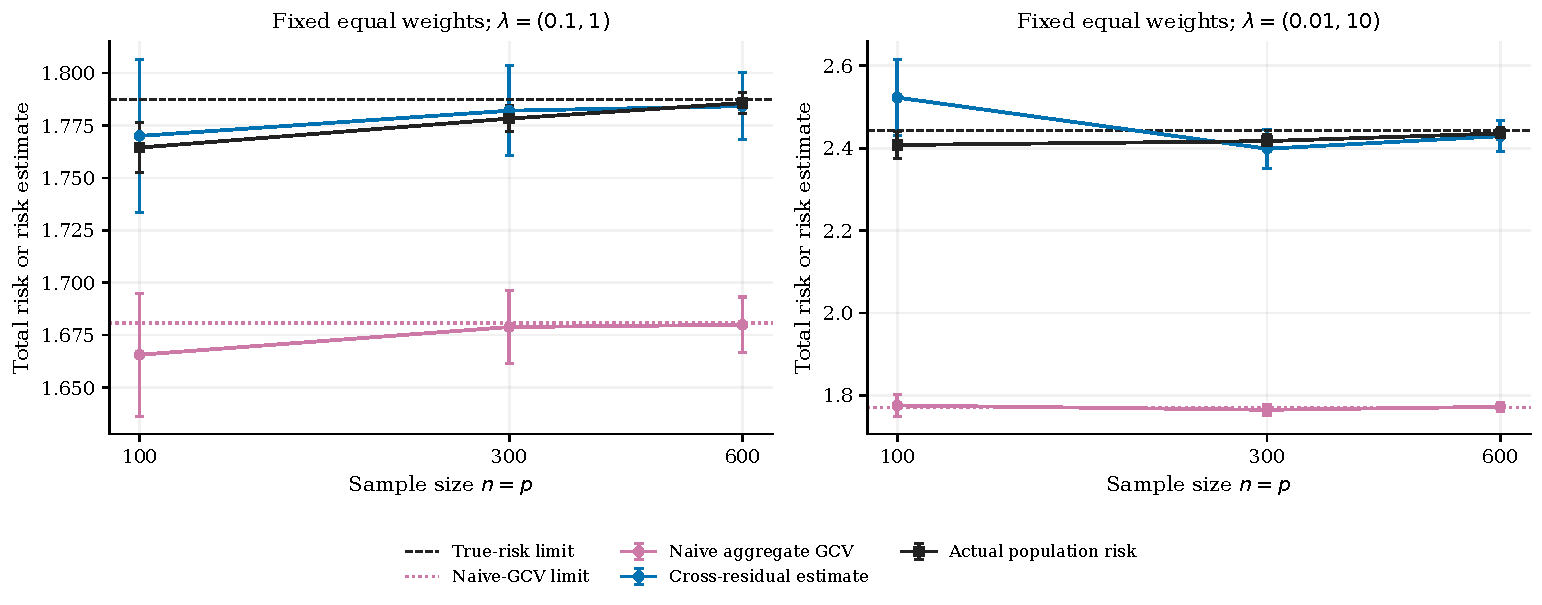
\includegraphics[width=\textwidth]{mp_validation.pdf}
\caption{固定权重 MP 验证：普通 GCV 与交叉残差估计随规模变化的均值及标准误，虚线为解析极限。
具体曲线含义见图例；这里没有数据选权。}\label{fig:mp}
\end{figure}
\begin{figure}[p]\centering
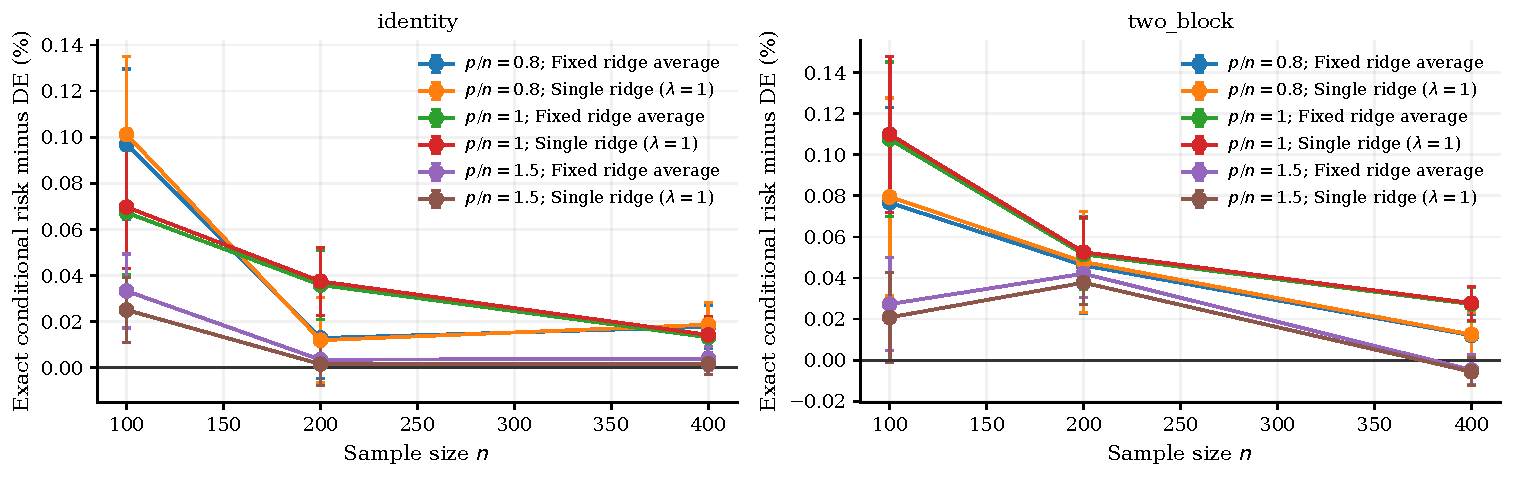
\includegraphics[width=\textwidth]{de_validation.pdf}
\caption{有界总体谱下的确定性等价验证。相对误差为精确条件风险减去谱方程预测，再除以预测值。
误差线为 $40$ 次独立设计上均值的 $\pm1\mathrm{SE}$；单个有限样本仍存在波动。}\label{fig:de}
\end{figure}
\clearpage
\section{研究边界与下一步应验收什么}
本阶段完成了理论基线、source alignment 的最小模拟、普通 GCV 失准机制和独立验证。
有限幂律模型中已观测到方法类收益，但幅度远小于实际权重估计损失。
因此后续优先问题应是稳定选权：例如限制有效候选维数、收缩到单岭或使用独立选权数据，
再检查是否能在明确场景中实现相对单岭的配对风险改善。
这些是后续待检验方案，本报告没有将其当作已实现结果。

本次没有证明一般各向异性双参数风险的完整确定性等价，
也没有证明候选数任意增长、正则下界趋零或无约束负权重下的统一一致性。
数学附录只在明确的固定候选集、正则参数远离零及有界谱条件下陈述选权保证。
所有模拟均为高斯设计、线性响应；结果尚未扩展到重尾数据或真实数据。
最小范数在插值点的重尾样本另存分位数与最大值，不能用其不稳定样本均值包装风险改进。

\section{交付清单与复现入口}
\begin{itemize}
\item \texttt{Code/}：风险与求解模块、主实验、独立渐近验证、统计绘图、结果核查、报告生成与单元测试。
\item \texttt{Results/}：逐次风险、逐候选权重、配对差值、条件 oracle 收益、校准、机制记录、种子清单与求解审计。
\item \texttt{Figures/}：六组矢量 PDF 图，另附 SVG 与 PNG；最小范数的尾部分布作为补充材料。
\item \texttt{Report/}：本 PDF、可编辑完整 \LaTeX{} 源文件、数学片段和文献条件说明。
\item 项目根目录的 \texttt{README.md}、\texttt{requirements.txt}、\texttt{run\_all.sh} 给出完整复现顺序。
\end{itemize}
本次执行使用 Python 3.12.14、NumPy 2.5.4、SciPy 1.18.1。
所需依赖均在清单中固定版本，报告由 XeLaTeX 实际编译。

\clearpage
\appendix
% Standalone content fragment. Requires amsmath, amssymb, hyperref.
% Citation keys: dw, richards, bellec, bach, wu, lin.
\section{数学对象与两个不同的风险目标}\label{sec:theory_setup}
设 $X\in\mathbb R^{n\times p}$ 的行为训练特征，$y=X\beta+\varepsilon$。
训练噪声满足 $\mathbb E\varepsilon=0$、$\operatorname{Cov}(\varepsilon)=\sigma^2I_n$，$0<\sigma^2<\infty$，
与系数及设计独立；新特征 $x_0$ 均值为零、协方差为 $\Sigma\succeq0$，
新噪声方差同为 $\sigma^2$，且测试点独立于训练数据。
采用规范化岭损失 $\lVert y-Xb\rVert_2^2/n+\lambda\lVert b\rVert_2^2$，记
\begin{equation}\label{eq:th_ridge}
 S=X^{\mathsf T}X/n,\quad Q_j=(S+\lambda_jI_p)^{-1},\quad
 \widehat\beta_j=Q_jX^{\mathsf T}y/n,\qquad \lambda_j>0.
\end{equation}
候选数为 $K$，混合权重满足 $\boldsymbol1^{\mathsf T}\pi=1$，
估计器为 $\widehat\beta_\pi=\sum_{j=1}^K\pi_j\widehat\beta_j$。

\textbf{给定真实系数和训练结果的风险。}
以 $\mathcal D=(X,y)$ 表示训练数据，定义
\begin{align}
 R_{\mathcal D}(\pi)
 &=\mathbb E[(y_0-x_0^{\mathsf T}\widehat\beta_\pi)^2\mid X,y,\beta]
 =\pi^{\mathsf T}\mathcal K_{\mathcal D}\pi,\label{eq:th_realized_risk}\\
 (\mathcal K_{\mathcal D})_{jk}
 &=\sigma^2+(\widehat\beta_j-\beta)^{\mathsf T}\Sigma(\widehat\beta_k-\beta).
 \label{eq:th_realized_matrix}
\end{align}
它可以用于模拟中的精确总体评估，不需要另抽有限测试集；真实系数仅供评估，不能进入实际选权。
如果以式\eqref{eq:th_realized_matrix}选权，则得到使用真实系数的事后 oracle。

\textbf{给定设计、对系数与训练噪声平均的风险。}
另设 $\mathbb E\beta=0$、$\operatorname{Cov}(\beta)=\Psi\succeq0$，且 $\beta$ 与 $X$ 独立。
对固定权重或仅依赖 $X$ 的权重，定义
$\overline R_X(\pi)=\mathbb E_{\beta,\varepsilon}[R_{\mathcal D}(\pi)\mid X]$。
用此目标选权的 oracle 可知道生成参数 $\Sigma,\Psi,\sigma^2$，但不使用某一次真实系数或噪声的实现值。
两个 oracle 的信息与目标不同，不能混为同一个基准。

\paragraph{命题 1：一般先验下的精确交叉风险。}
在上述二阶矩条件下，
\begin{align}
 \overline R_X(\pi)&=\sigma^2+\pi^{\mathsf T}C_X\pi,\label{eq:th_prior_risk}\\
 (C_X)_{jk}
 &=\lambda_j\lambda_k\operatorname{tr}(\Sigma Q_j\Psi Q_k)
   +\frac{\sigma^2}{n}\operatorname{tr}(\Sigma SQ_jQ_k).
 \label{eq:th_prior_matrix}
\end{align}
矩阵 $C_X$ 对称半正定；式\eqref{eq:th_prior_matrix}不要求 $\Sigma,\Psi,S$ 可交换。

\textit{证明。}
由 $Q_jS=I_p-\lambda_jQ_j$ 和权重和为一，
\begin{equation}\label{eq:th_error_decomp}
 \widehat\beta_\pi-\beta
 =-\left(\sum_j\pi_j\lambda_jQ_j\right)\beta
  +\left(\sum_j\pi_jQ_j\right)X^{\mathsf T}\varepsilon/n.
\end{equation}
两项交叉期望为零。偏差项用 $\mathbb E\beta\beta^{\mathsf T}=\Psi$ 展开，
噪声项用 $\mathbb E\varepsilon\varepsilon^{\mathsf T}=\sigma^2I_n$ 展开，
即得式\eqref{eq:th_prior_matrix}。任意线性组合的对应二次型是两个非负方差项之和，故半正定。
若 $\widehat\pi$ 依赖 $y$，不能把它直接代入固定权重的式\eqref{eq:th_prior_risk}，
并将结果认作 $\mathbb E[R_{\mathcal D}(\widehat\pi)\mid X]$。
\hfill$\square$

\subsection{各向同性情形的差商与高维极限}
当 $\Psi=\alpha^2I_p/p$ 时，令 $t_p(\lambda)=p^{-1}\operatorname{tr}[\Sigma(S+\lambda I_p)^{-1}]$。
先设候选参数两两不同。对 $j\ne k$ 定义
\begin{align}
 B_{jk}&=\frac{t_p(\lambda_j)-t_p(\lambda_k)}{\lambda_k-\lambda_j},&
 V_{jk}&=\frac{\lambda_kt_p(\lambda_k)-\lambda_jt_p(\lambda_j)}{\lambda_k-\lambda_j},\label{eq:th_divided}\\
 B_{jj}&=-t_p'(\lambda_j),&
 V_{jj}&=t_p(\lambda_j)+\lambda_jt_p'(\lambda_j).
 \label{eq:th_diag}
\end{align}
那么
\begin{equation}\label{eq:th_isotropic_matrix}
 (C_X)_{jk}=\alpha^2\lambda_j\lambda_kB_{jk}+\sigma^2(p/n)V_{jk}.
\end{equation}
其证明分别使用
$Q_jQ_k=(Q_j-Q_k)/(\lambda_k-\lambda_j)$ 和
$SQ_jQ_k=(\lambda_kQ_k-\lambda_jQ_j)/(\lambda_k-\lambda_j)$，对角取连续极限。
后者说明方差交叉项包含样本协方差 $S$，不能与偏差交叉项混用。

在 Dobriban--Wager 的比例高维条件下\cite{dw}，例如
$p/n\to\gamma\in(0,\infty)$、$X=Z\Sigma^{1/2}$、$Z$ 元素独立同分布、均值零、方差一且十二阶矩一致有界、
$\lVert\Sigma\rVert_{\mathrm{op}}$ 一致有界、总体经验谱弱收敛到 $H$，
对固定有限候选集、固定 $\lambda_j>0$，可用极限 $t$ 及其导数替换式\eqref{eq:th_divided}--\eqref{eq:th_diag}中的 $t_p$。
其中 $v_\lambda>0$ 解
\begin{equation}\label{eq:th_stieltjes}
 \frac1{v_\lambda}=\lambda+\gamma\int\frac{s}{1+sv_\lambda}\,dH(s),\qquad
 t(\lambda)=\frac1\gamma\left(\frac1{\lambda v_\lambda}-1\right).
\end{equation}
这是现有随机矩阵结论与 resolvent 恒等式的组合，不作为新定理宣称。
一般 $\Psi$ 的偏差项为 $\operatorname{tr}(\Sigma Q_j\Psi Q_k)$，
即使 $\Psi$ 与总体 $\Sigma$ 同时对角化，也通常不与样本 $Q_j$ 交换，因而不能直接使用上述单函数差商。
本项目对一般 $\Psi$ 使用式\eqref{eq:th_prior_matrix}的精确有限样本计算；
一般 source condition 的渐近分析需要另行引用与验证\cite{richards,wu}。

\section{连续最优单岭与平均收益的正确基准}\label{sec:theory_bayes}
\paragraph{命题 2：各向同性二阶矩下的最优线性基准。}
给定 $X$，设 $\Psi=\alpha^2I_p/p$，$\alpha^2,\sigma^2>0$，
令 $V_y=(\alpha^2/p)XX^{\mathsf T}+\sigma^2I_n$。
在全部仅依赖 $X$ 的线性估计器 $Ay$ 中，
\begin{equation}\label{eq:th_lmmse}
 A_*=(\alpha^2/p)X^{\mathsf T}V_y^{-1}
 =(X^{\mathsf T}X+n\lambda_*I_p)^{-1}X^{\mathsf T},\qquad
 \lambda_*=(p/n)\sigma^2/\alpha^2
\end{equation}
具有最小先验平均预测风险，而且
\begin{equation}\label{eq:th_lmmse_gap}
 \overline R_X(A)-\overline R_X(A_*)
 =\operatorname{tr}\!\left[\Sigma(A-A_*)V_y(A-A_*)^{\mathsf T}\right]\ge0.
\end{equation}

\textit{证明。}
$\operatorname{Cov}(\beta-A_*y,y\mid X)=(\alpha^2/p)X^{\mathsf T}-A_*V_y=0$。
将 $Ay-\beta=(A_*y-\beta)+(A-A_*)y$ 的加权平方展开，交叉期望为零，余项即式\eqref{eq:th_lmmse_gap}。
若系数和噪声进一步为独立高斯，$A_*y$ 就是后验均值；
平方损失的条件期望分解将该最优性扩展到全部使用同样 $X,y$ 的估计器，包括依赖 $y$ 的选权。
仅有二阶矩而无高斯假设时，不宣称这个更强结论。
\hfill$\square$

据此，须分别报告平均相对\emph{离散网格最佳单岭}与\emph{连续调参最佳单岭}的差距。
网格未包含 $\lambda_*$ 时，正确先验下平均也可能改善离散网格的最佳值；
先验各向异性后不再有上述普遍的标量岭最优保证，但这并不保证任何给定平均家族都有严格收益。
例如 $S=sI_p$ 时，任意正岭的凸平均仍等价于某个单岭的标量收缩。
使用真实系数的事后 oracle 不属于式\eqref{eq:th_lmmse}的信息范围。

\section{普通聚合 GCV 与交叉残差准则的精确关系}\label{sec:theory_gcv}
记
\begin{equation}\label{eq:th_gcv_notation}
 H_j=XQ_jX^{\mathsf T}/n,\quad r_j=(I_n-H_j)y,\quad
 d_j=1-\operatorname{tr}(H_j)/n,\quad
 \mathsf E=(r_1,\ldots,r_K),\quad D=\operatorname{diag}(d_1,\ldots,d_K).
\end{equation}
正的岭参数保证 $d_j>0$。
以下以 $d=(d_1,\ldots,d_K)^{\mathsf T}$ 表示这些分量构成的向量。
本文所称普通聚合 GCV 与交叉残差矩阵分别为
\begin{align}
 G_{\mathrm{agg}}(\pi)
 &=\frac{\lVert\mathsf E\pi\rVert_2^2/n}{(d^{\mathsf T}\pi)^2},\label{eq:th_agg_gcv}\\
 \widehat{\mathcal K}
 &=D^{-1}\mathsf E^{\mathsf T}\mathsf E D^{-1}/n,\qquad
 G_{\mathrm{cross}}(\pi)=\pi^{\mathsf T}\widehat{\mathcal K}\pi.
 \label{eq:th_cross_gcv}
\end{align}
式\eqref{eq:th_cross_gcv}是既有交叉风险校正框架在完整数据上的形式\cite{bellec}，不作为新方法宣称。
固定权重时，删点并保持惩罚总量 $n\lambda_j$ 不变，逐候选重拟合的 LOO 残差是
\begin{equation}\label{eq:th_loo}
 r_i^{\mathrm{LOO,MA}}=\sum_j\pi_j\frac{r_{j,i}}{1-H_{j,ii}}.
\end{equation}
这是固定权重候选集合的 LOO 准则；若要计算整个自适应选权流程的外层 LOO，还需在删点后重新选权。

\paragraph{命题 3：同一个二次规划可以产生不同的实际模型。}
在单纯形 $\Delta_K=\{\pi\ge0:\boldsymbol1^{\mathsf T}\pi=1\}$ 上，变换
\begin{equation}\label{eq:th_gcv_map}
 u_j=\frac{d_j\pi_j}{d^{\mathsf T}\pi},\qquad
 \pi_j=\frac{u_j/d_j}{\sum_k u_k/d_k}
\end{equation}
是双射，并且
\begin{equation}\label{eq:th_gcv_equiv}
 G_{\mathrm{agg}}(\pi)=u^{\mathsf T}\widehat{\mathcal K}u,\qquad
 \min_{\pi\in\Delta_K}G_{\mathrm{agg}}(\pi)
 =\min_{u\in\Delta_K}G_{\mathrm{cross}}(u).
\end{equation}

\textit{证明。}
$d_j>0$ 保证变换及其逆均将单纯形映到单纯形。
由 $D^{-1}u=\pi/(d^{\mathsf T}\pi)$ 代入式\eqref{eq:th_cross_gcv}，即得等式。
\hfill$\square$

因此，两种优化的最小分数可以完全相同，但普通 GCV 使用的实际权重为 $\pi$，
交叉残差准则使用的实际权重为 $u$。
对正权重分量，$\pi_j/\pi_k=(u_j/u_k)(d_k/d_j)$；
较小 $d_j$ 对应更高自由度，逆变换会提高这些分量的相对比重。
这给出一个无需渐近分析的机制，但并不保证每份数据上普通 GCV 的实际风险都更高。
该变换一般不保持有负权重时的 $\ell_1$ 约束，也可能遇到 $d^{\mathsf T}\pi=0$，故不能原样推广到负权重优化。
这一命题是本项目采用的代数解释；未进行穷尽查新，不据此宣称首次发现。

\subsection{固定权重下普通 GCV 不一致的显式例子}
取独立标准高斯设计，$p/n\to1$，$\Sigma=I_p$，
$\beta\sim N(0,I_p/p)$、$\varepsilon\sim N(0,I_n)$ 相互独立，
固定 $\pi=(1/2,1/2)$。
令 $F$ 为比例一的 Marchenko--Pastur 分布，
$u_0(s)=\sum_j\pi_j\lambda_j/(s+\lambda_j)$。
预测风险与普通 GCV 分别收敛到
\begin{align}
 R_\infty
 &=1+\int\left[u_0(s)^2+\frac{(1-u_0(s))^2}{s}\right]dF(s),\label{eq:th_mp_risk}\\
 G_{\mathrm{agg},\infty}
 &=\frac{\int(s+1)u_0(s)^2\,dF(s)}{\left[\int u_0(s)\,dF(s)\right]^2}.
 \label{eq:th_mp_gcv}
\end{align}
第一式由式\eqref{eq:th_isotropic_matrix}得到；
第二式来自 $y$ 在训练样本谱基中的条件协方差 $XX^{\mathsf T}/p+I_n$。
利用 $t(\lambda)=(\sqrt{1+4/\lambda}-1)/2$，
当 $\lambda=(0.1,1)$ 时二者分别为 $1.787525057$ 和 $1.680756692$；
当 $\lambda=(0.01,10)$ 时分别为 $2.443469136$ 和 $1.769954995$。
这已经是在固定权重下的差异，与额外的数据选权过拟合是不同问题。

\section{受约束选权的稳定性保证与适用范围}\label{sec:theory_stability}
对 $L\ge1$，定义非空紧权重集合
\begin{equation}\label{eq:th_weight_class}
 \mathcal W_L=\{\pi\in\mathbb R^K:\boldsymbol1^{\mathsf T}\pi=1,\ \lVert\pi\rVert_1\le L\}.
\end{equation}
特别地 $\mathcal W_1=\Delta_K$；$L>1$ 允许负权重。

\paragraph{命题 4：矩阵误差到选权误差的确定性传递。}
对任意对称矩阵 $\mathcal K,\widehat{\mathcal K}$，令
$\epsilon=\max_{j,k}|\widehat{\mathcal K}_{jk}-\mathcal K_{jk}|$。
若数值解 $\widehat\pi\in\mathcal W_L$ 满足
$\widehat\pi^{\mathsf T}\widehat{\mathcal K}\widehat\pi
\le\inf_{\pi\in\mathcal W_L}\pi^{\mathsf T}\widehat{\mathcal K}\pi+\delta_{\mathrm{opt}}$，则
\begin{align}
 \sup_{\pi\in\mathcal W_L}
 |\pi^{\mathsf T}(\widehat{\mathcal K}-\mathcal K)\pi|
 &\le L^2\epsilon,\label{eq:th_uniform_bound}\\
 \widehat\pi^{\mathsf T}\mathcal K\widehat\pi
 -\inf_{\pi\in\mathcal W_L}\pi^{\mathsf T}\mathcal K\pi
 &\le 2L^2\epsilon+\delta_{\mathrm{opt}}.
 \label{eq:th_oracle_bound}
\end{align}

\textit{证明。}
逐项取绝对值得
$|\sum_{jk}\pi_j\pi_k(\widehat{\mathcal K}-\mathcal K)_{jk}|
\le\epsilon(\sum_j|\pi_j|)^2\le L^2\epsilon$。
在估计最小值和真实最小值之间加减两个估计二次型，分别用此界与优化误差，即得第二式。
\hfill$\square$

这个界本身不说明 $\epsilon\to0$。它说明无约束放大负权重会同步放大风险估计误差；
$L=3$ 的界常数是 $L=1$ 时的九倍，而非免费的模型类扩张。

\paragraph{推论 1：已有交叉风险界可支持的固定候选集结论。}
考虑一列高斯线性回归问题：$x_i\sim N(0,\Sigma_n)$，独立噪声为 $N(0,\sigma^2)$，
$\sup_n p/n<\infty$、$\sup_n\lVert\Sigma_n\rVert_{\mathrm{op}}<\infty$；
固定 $K,L$，确定性候选参数满足
$0<\underline\lambda\le\lambda_j\le\overline\lambda<\infty$。
令固定系数满足 $\sup_n\beta_n^{\mathsf T}\Sigma_n\beta_n<\infty$。
则式\eqref{eq:th_cross_gcv}的估计矩阵对式\eqref{eq:th_realized_matrix}满足
\begin{equation}\label{eq:th_cross_rate}
 \max_{j,k}|\widehat{\mathcal K}_{jk}-(\mathcal K_{\mathcal D})_{jk}|
 =O_{\mathbb P}(n^{-1/2}),
\end{equation}
因此在数值优化误差为 $o_{\mathbb P}(1)$ 时，
\begin{equation}\label{eq:th_cross_consistency}
 R_{\mathcal D}(\widehat\pi)-\inf_{\pi\in\mathcal W_L}R_{\mathcal D}(\pi)
 =O_{\mathbb P}(L^2n^{-1/2})+\delta_{\mathrm{opt}}=o_{\mathbb P}(1).
\end{equation}
这里的 oracle 目标是给定真实系数与训练结果的 $R_{\mathcal D}$，不是先验平均 $\overline R_X$。

\textit{推导与引用边界。}
使用 Bellec 等人交叉风险非渐近界\cite{bellec}的 Theorem 1、式 (20)，
取完整数据 $I_j=[n]$；这个逐对界允许不同的惩罚 $g_j(b)=\lambda_j\lVert b\rVert_2^2/2$。
在上述条件下，它给出
\begin{equation}\label{eq:th_cited_cross_bound}
 \mathbb E\left[
 d_jd_k\frac{|\widehat{\mathcal K}_{jk}-(\mathcal K_{\mathcal D})_{jk}|}
 {\sqrt{(\mathcal K_{\mathcal D})_{jj}(\mathcal K_{\mathcal D})_{kk}}}
 \right]\le\frac{C_0}{\sqrt n},
\end{equation}
其中 $C_0$ 可依赖固定的比例、谱和正则界。高斯设计给出 $\lVert S\rVert_{\mathrm{op}}=O_{\mathbb P}(1)$，
而 $d_j\ge\underline\lambda/(\lVert S\rVert_{\mathrm{op}}+\underline\lambda)$，故所有 $d_j$ 以高概率远离零。
由岭线性算子的奇异值界，
$\lVert\widehat\beta_j\rVert_2\le\lVert y\rVert_2/(2\sqrt{n\underline\lambda})$；
再用 $\lVert y\rVert_2^2/n=O_{\mathbb P}(1)$ 可得 $(\mathcal K_{\mathcal D})_{jj}=O_{\mathbb P}(1)$。
式\eqref{eq:th_cited_cross_bound}、Markov 不等式与固定有限个指标的并界得到式\eqref{eq:th_cross_rate}；
最后应用命题 4。
对独立随机系数，只要 $\beta^{\mathsf T}\Sigma_n\beta=O_{\mathbb P}(1)$，同样可条件化使用这个论证。

这是一条由现有逐对估计界与确定性误差传递得到的受限推论，不是对任意候选数、任意负权重或 $\lambda\to0$ 的完整一致性定理。
尤其不能把文献中随机子样本、共同惩罚的普通 GCV 不一致定理，原样当作同一设计不同 $\lambda$ 的定理。
式\eqref{eq:th_cited_cross_bound}的逐对结果足以用于这里的固定候选集，但须核查所用完整数据矩阵和参数界。

\section{信号谱对齐、滤波器限制与本次结论的范围}\label{sec:theory_source}
设总体协方差的特征对为 $(\mu_i,v_i)$，$\mu_i\asymp i^{-a}$，$a>1$。
参照 source condition，令
\begin{equation}\label{eq:th_source_condition}
 \mathbb E\langle v_i,\beta\rangle\langle v_j,\beta\rangle=0\ (i\ne j),\qquad
 \mu_i\mathbb E\langle v_i,\beta\rangle^2\asymp i^{-b}.
\end{equation}
这里是对先验的二阶矩条件，不是某一次随机系数的逐坐标等式\cite{lin,richards}。
相应系数方差与 $i^{a-b}$ 成比例；$b=a$ 对应各向同性，
$b<a$ 相对提高弱谱方向的系数方差，$b>a$ 相对强调强谱方向。
比较 $b$ 时固定 $\operatorname{tr}(\Sigma\Psi)/\sigma^2$，才能排除总预测信号能量变化的影响。
响应机制仍为正确线性模型，故应称为先验或正则结构变化，而非自动称线性模型误设。

在样本谱值 $s\ge0$ 上，平均岭的拟合滤波器为
\begin{equation}\label{eq:th_filter}
 h_\pi(s)=\sum_j\pi_j\frac{s}{s+\lambda_j}.
\end{equation}
凸权重下 $h_\pi'(s)>0$、$h_\pi''(s)<0$；允许负权重可解除这些形状限制，
但固定有限 $K$ 时仍只是带固定极点的有理函数族，满足 $h_\pi(0)=0$、$h_\pi(\infty)=1$。
它不能恢复训练设计零空间中的系数，扩大滤波器家族也不等于自动获得可实现的低风险选权。
跨岭参数的外推与加权正则化已有直接研究\cite{bach,wu}，本报告不把这些组合本身称为首次提出。

\textbf{有限维实验与渐近保证的区别。}
若将截断幂律谱重新规范到 $\operatorname{tr}(\Sigma)=p$，其最大特征值会随 $p$ 增长，
通常不满足上述一致有界谱假设；若不重标，经验谱又可能退化。
因此本次有限维机制实验的精确风险矩阵始终有效，但它不能单独证明无限维 Scaling Law，
也不能将推论 1 的一致性保证无条件外推到该幂律增维路径。
本次可争取的结果是：确认一般先验的有限样本风险基线，分开测量网格收益、模型类收益和实际选权代价，
并在满足明确假设的固定候选集上陈述可证明的稳定性结论。

\clearpage
\begin{thebibliography}{7}\small
\bibitem{dw} Dobriban, E. and Wager, S. (2018). \href{https://arxiv.org/abs/1507.03003}{High-Dimensional Asymptotics of Prediction: Ridge Regression and Classification}. \emph{Annals of Statistics}, 46(1), 247--279.
\bibitem{richards} Richards, D., Mourtada, J. and Rosasco, L. (2021). \href{https://proceedings.mlr.press/v130/richards21b.html}{Asymptotics of Ridge(less) Regression under General Source Condition}. \emph{AISTATS}, PMLR 130, 3889--3897.
\bibitem{bellec} Bellec, P. C., Du, J.-H., Koriyama, T., Patil, P. and Tan, K. (2025). \href{https://arxiv.org/html/2310.01374v2}{Corrected generalized cross-validation for finite ensembles of penalized estimators}. \emph{JRSSB}, 87(2), 289--318.
\bibitem{bach} Bach, F. (2021). \href{https://www.di.ens.fr/~fbach/Richardson_SIAM_2021.pdf}{On the Effectiveness of Richardson Extrapolation in Data Science}. \emph{SIAM Journal on Mathematics of Data Science}, 3(4), 1251--1277.
\bibitem{wu} Wu, D. and Xu, J. (2020). \href{https://proceedings.neurips.cc/paper/2020/hash/72e6d3238361fe70f22fb0ac624a7072-Abstract.html}{On the Optimal Weighted $\ell_2$ Regularization in Overparameterized Linear Regression}. \emph{NeurIPS} 33.
\bibitem{lin} Lin, L., Wu, J., Kakade, S. M., Bartlett, P. L. and Lee, J. D. (2024). \href{https://proceedings.neurips.cc/paper_files/paper/2024/hash/6fcb1afcc1e9c2c82c8ddddf03bcf0f6-Abstract.html}{Scaling Laws in Linear Regression: Compute, Parameters, and Data}. \emph{NeurIPS} 37.
\bibitem{zhao} Zhao, S., Liao, J. and Yu, D. (2020; online 2018). \href{https://link.springer.com/article/10.1007/s00362-018-1002-4}{Model averaging estimator in ridge regression and its large sample properties}. \emph{Statistical Papers}, 61, 1719--1739.
\end{thebibliography}
\end{document}
